\documentclass{standalone}

\usepackage{tikz}
\usepackage{standalone}
\usetikzlibrary{calc}

\begin{document}
    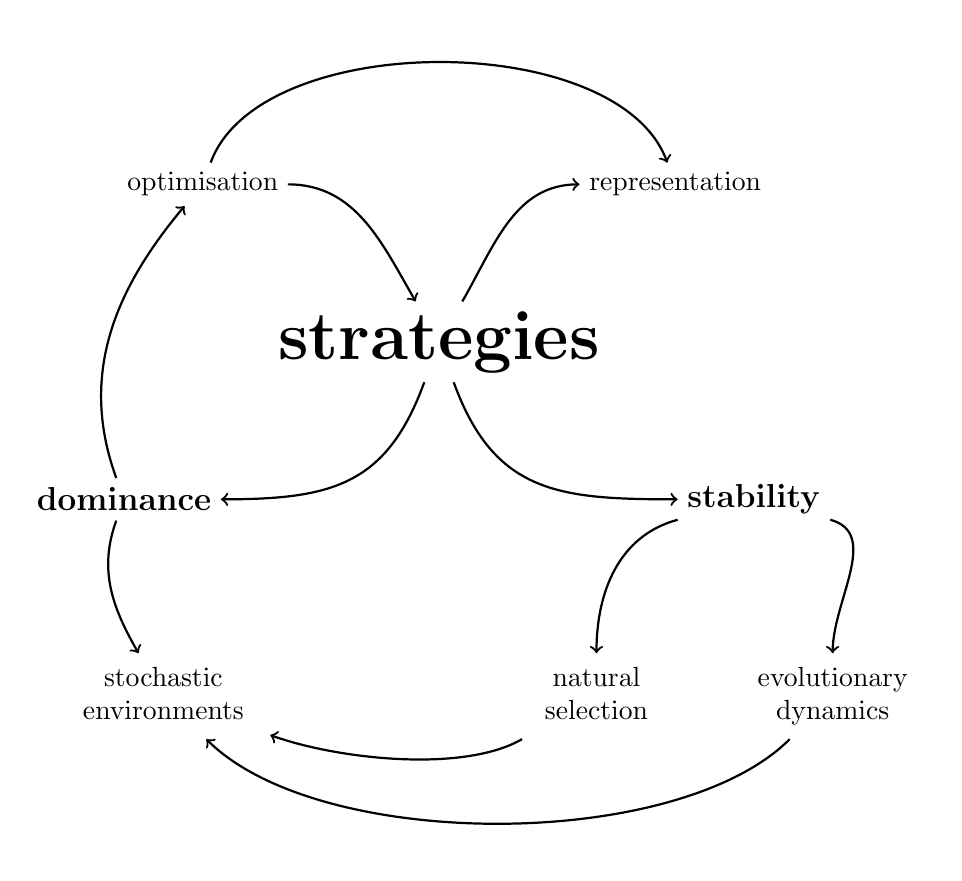
\begin{tikzpicture}

    \tikzstyle{state}=[minimum width=0.8cm, font=\boldmath];


    \node (6) at (-3, 2) [state] {optimisation};
    \node (0) at (0, 0) [state]	{\Huge\textbf{strategies}};
    \node (7) at (3, 2) [state] {representation};
    \node (1) at (-4, -2) [state]	{\large\textbf{dominance}};

    \draw (6) edge[out=0, in=120, ->, thick] node {} (0);
    \draw (0) edge[out=-110, in=0, ->, thick, looseness=1.2] node {} (1);
    \draw (1) edge[out=110, in=-130, ->, thick] node {} (6);
    \draw (6) edge[out=70, in=110, ->, thick, looseness=0.8] node {} (7);
    \draw (0) edge[out=60, in=180, ->, thick] node {} (7);

    \node (2) at (4, -2) [state]	{\large\textbf{stability}};
    \node (3) at (2, -4.5) [state]  {\begin{tabular}{c} natural 
                  \\ selection \end{tabular}};
    \node (4) at (5, -4.5) [state]	{\begin{tabular}{c} evolutionary 
			\\ dynamics \end{tabular}};
    % \node (5) at (7, -3) [state] {spatial};
    % \node (8) at (6, -5) [state] {moran process};

    \draw (0) edge[out=-70, in=180, ->, thick, looseness=1.2] node {} (2);
    \draw (2) edge[out=-165, in=90, ->, thick] node {} (3);
    \draw (2) edge[out=-15, in=90, ->, thick] node {} (4);
    % \draw (4) edge[out=10, in=180, ->, thick] node {} (5);
    % \draw (4) edge[out=-200 in=90, ->, thick] node {} (8);

    \node (9) at (-3.5, -4.5) [state]	{\begin{tabular}{c} stochastic 
								  \\ environments \end{tabular}};

    \draw (1) edge[out=-110, in=120, ->, thick] node {} (9);
    \draw (3) edge[out=-150, in=-20, ->, thick, looseness=.7] node {} (9);
    \draw (4) edge[out=-135, in=-45, ->, thick, looseness=0.7] node {} (9);
    \end{tikzpicture}
\end{document}